% !Mode:: "TeX:UTF-8"

\documentclass[literaturereview]{zjutreport}

\graphicspath{{figures/}}  % 定义所有的eps文件在 figures 子目录下
\begin{document}           % 开始全文

%论文题目:{中文}
\zjuttitle{浙江工业大学本科生毕业设计文献综述模板}
%作者:{中文姓名}{学号}
\zjutauthor{徐呵呵}{200926399999}
%指导教师:{导师中文名}
\zjutmentor{王~~~~哈}
%个人信息:{毕业年份}{专业班级}
\zjutinfo{2013}{计算机科学与技术0905}
%学院信息:{学院中文}
\zjutcollege{计算机科学与技术学院}
%日期:{提交日期}
\zjutdate{2013年06月}

% !Mode:: "TeX:UTF-8"
%%============================================================
%% 中文封面

\thispagestyle{empty}
\pdfbookmark[-1]{\zjuttitlec}{zjutthesiscover}
\phantomsection \label{zjutthesiscover}
\vspace*{4mm}
% 校名
\begin{center}
   \includegraphics[width=98.40mm]{figures/zjut}
\end{center}
\vspace*{12mm}
\centerline{\songti\yihao{本科毕业设计说明书(论文)}}
\vspace*{8mm}
\centerline{\songti\xiaoer\textbf{(\zjutgrade\ 届)}}
\vspace*{7mm}
% 校徽
\begin{center}
  \includegraphics[width=27.3mm]{figures/zjutlogo}
\end{center}

\vspace*{0.0mm}
\renewcommand{\arraystretch}{1.0}
\hspace*{12mm} 
{\songti\erhao{论文题目}}
\hspace{6mm} 
\begin{minipage}[t]{85mm} % 这里建议自行微调
    \linespread{1.1}{\songti\xiaoer\CJKunderline*{\zjuttitlec}}
\end{minipage}
\vspace*{1mm}
\begin{center}
    \setlength{\arrayrulewidth}{0.5pt}
    {\songti\sihao
        \renewcommand{\arraystretch}{1}
        \begin{tabular}{lc}
            作者姓名\qquad &  \zjutauthornamec \\ \cline{2-2}
            指导教师\qquad &  \zjutmentorc\\ \cline{2-2}
            \\
            学科(专业)\qquad &  \zjutmajor \\ \cline{2-2}
            所在学院\qquad &  \zjutcollegec \\ \cline{2-2}
            提交日期\qquad & \zjutsubmitteddatee \\ \cline{2-2}
        \end{tabular}
    }
\end{center}

      % 封面

\frontmatter

\pagenumbering{Roman}
\begingroup % 在组内的chapter不换行
\let\clearpage\relax % chapter之后不换页

%%%%%%%%%% 标题 %%%%%%%%%%
\vspace*{3.0mm}
\centerline{\sanhao\heiti\bfseries\zjuttitlec}
\vspace*{3.0mm}

%%%%%%%%%% 摘要 %%%%%%%%%%
\include{preface/abstract}     % 中文摘要

%%%%%%%%%% 正文 %%%%%%%%%%
\mainmatter
% \makeatletter
% !Mode:: "TeX:UTF-8"

\chapter{绪论}
\section{研究背景及意义}

魔方作为凝聚了人类智慧的玩具,不仅可以培养人们的空间想象力、记忆力等,更可以锻炼手脑协同工作能力,其还原过程代表着人类三维空间想象及逻辑推理运算等方面的智力行为~\cite{1}~\cite{2}。再者,如今出现以不同方式还原魔方的竞技运动,例如单手还原魔方、双手还原魔方等。可见在解魔方这个过程中,人们有各式各样的办法与招式。而标准三阶魔方可称得上是所有魔方类型中的经典。如下图~\ref{fig:1-1}~是一个标准的三阶魔方实例图。

\begin{figure}[H]
	\centering
	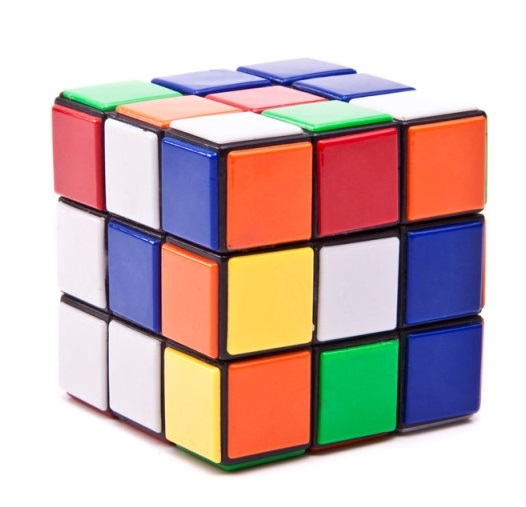
\includegraphics[width=0.4\textwidth]{1-1}
	\caption{标准三阶魔方}\label{fig:1-1}
\end{figure}

近年来,研究人员开始考虑研究魔方还原的机器人自动化设备以追求魔方复原速度上的极致。对于魔方还原的机器人自动化设备,其技术关键是如何设计复原操作装置、颜色识别算法以及魔方复原算法来可靠地完成复原任务。这正是本论文研究所需要解决的问题。本论文借助Arduino嵌入式系统开发魔方还原系统~\cite{3}~\cite{4},不仅可以极大地简化开发步骤,而且能够提高还原效率。本系统经过复杂的计算与推理,寻找还原步骤简化规律,可快速建立最优的还原操作;同时依次通过颜色识别模块、还原求解模块、串口通讯模块和电机转动模块可实现对任意打乱状态下的魔方进行精准、快速地还原。

\section{国内外研究现状}

早在1978年,匈牙利的数学家们把魔方介绍给当年国际数学家代表会的专家学者,这是魔方在数学家面前的首次正式亮相,同时也引起了极大的反响,受到了人们的广泛关注。
在随后的一段时间里英国便出现了历史上第一批的魔方理论研究小组。在1981年3月,魔方首次登上了《科学美国人》的封面。在魔方领域的众多概念中,魔方复原所需的最小转动次数称为“上帝之数”,也就是至少需要经过多少旋转操作能够复原一个打乱的魔方~\cite{1}。
“上帝之数”的具体数值吸引了非常多的魔方研究者~\cite{5},其中有相当一部分是数学家。数学家们用几十年的研究证明,任何打乱都可以在二十步内解决,即上帝之数为二十~\cite{6}。

近年来,魔方复原系统机器人引起了国内外研究人员的广泛兴趣。在国外,最早出现的魔方复原系统是在2010年世界制造者博览会上展出的名为“The Cubinator”的双臂魔方还原机器人,这款机器人是皮特-雷蒙德设计的,其工作原理是由相互垂直、呈九十度角的两个机械手臂旋转配合,通过一系列机械手臂对魔方的松紧操作,从而完成魔方复原。2011年,斯威本科技大学的一个学生小组研制了一款名为Ruby的魔方复原机器人,被人们誉为“最快魔方机械手”,该魔方机器人以10.96 s的成绩打破当时机器人复原魔方的最快纪录。2014年,由ARM的两位工程师完成的CubeStormer3机器人还原魔方仅需3.253秒,而上一代产品CubeStormer2需要5.27秒,并且当时人类复原魔方的记录则为5.5秒,机器人复原魔方的水平已远远领先人类的水平,该机器人的旋转部分采用的是四个与乐高机器人配对的伺服电机,机器人采用ARM驱动的三星Galaxy S4智能手机,由三星Exynos 5 Octa应用处理器驱动,分析立方体,并指导四个机器人手进行旋转操作,ARM9处理器还为八块乐高 MINDSTORMS EV3积木提供动力,执行电机排序和控制。2019年,日本工程师Human Controller制作了一款自还原的魔方,该工程师把魔方内部“魔改”了一番,把原本是简单连接杆的核心改成了电子机械结构~\cite{7},其结构包含了电机、电线、电池等复杂机械结构,使得魔方拥有了自动化的基础,魔方在被打乱的过程中,其内部芯片会存储打乱的顺序,当魔方检测到一段时间没有发生人为转动时,则会自动开始按照打乱的顺序倒序进行相反方向旋转的操作。除此之外,随着科技水平的进步,德国工程师Albert Beer设计的名为“Sub 1 Reloaded”的魔方机器人是目前世界上魔方复原速度最快的机器人,能够在 0.637 秒的时间内完成任务,其主要结构为空间中相互垂直的6个旋转轴,该魔方机器人通过两张照片来识别魔方的色块样式,然后借助 Herbert Kociemba 发明的两阶段算法~\cite{8}来计算出一套解决方案,最终在英飞凌处理器的指挥下,让机械臂在1s内完成最后的操作。相比于文献\mycite{9}中介绍的魔方复原的算法,两阶段算法具有在复原步骤上有很明显的优势。

在国内,也有许多魔方爱好者设计了不同复原方式的魔方复原系统,例如用双臂解魔方机器人系统~\cite{10}~\cite{11}、四臂魔方还原系统~\cite{12}等,除此之外还有基于不同嵌入式平台的系统~\cite{13},例如基于FPGA异构平台的魔方还原系统~\cite{14}、基于ARM9的魔方机器人系统~\cite{15}、基于STM32的解魔方系统~\cite{11}~\cite{16}等。南通理工学院的解魔方机器人~\cite{17}可以在七十秒之内完成魔方的复原。北京理工大学珠海学院自动化学院设计的魔方还原系统采用双气动控制的方法,其魔方还原成功率可达到97\%~\cite{10}。济南大学的田田~\cite{18}~\cite{19}设计了一款同样基于气动的解魔方组合机械手,该方法通过采用带有CMOS图像传感器的摄像头来捕获各个魔方块的颜色图像,再通过RGB颜色模型完成魔方色块的颜色识别,以本地计算机为上位机,采用Thistlethwaite算法计算出复原步骤,最后通过控制气动机械手进行魔方复原。大连民族学院的董海洋~\cite{20}设计了一款通过四轴还原魔方的类人机械臂机器人,以安卓操作系统的智能机作为上位机,通过摄像头完成图像采集,并计算出还原指令,通过嵌入式控制板连接舵机,再接收客户端发出的还原指令,最终串行调度相互垂直的四个机械手臂,从而执行魔方复原动作。东北大学的张雪娇~\cite{21}设计了一款硬件部分由乐高组件组成的魔方机器人,该机器人采用能将光学影像转化为数字信号的CCD半导体作为图像采集模块,并使用笔记本电脑作为上位机对捕捉到的图像进行预处理与魔方块颜色识别。除此之外,国产魔方品牌GAN设计的全球消费级智能魔方机器人GAN Robot能在五秒内复原任意打乱的魔方。该机器人采用的是五轴伺服系统,由动力台、动力臂及X旋爪组成,四向卡位底座,固定动力臂。若要进行复原操作,则需要使用配套的魔方,并且在相应的APP平台上,其复原的原理是魔方中心轴记录打乱的顺序并通过蓝牙将其顺序发送到APP平台上,通过APP平台进行还原算法的推理,得出还原的顺序及各自的转动方向后将其发送到四向卡位底座进行还原。

随着上述各种魔方还原机器人的出现,也有越来越多的各界人士包括数学家们研究魔方还原算法,追求魔方还原在速度、效率上的极致。并且由于解魔方本身具有趣味性及可观赏性,研究解魔方的人也越来越多。

\section{本文的主要工作}

本文主要的研究目标是基于Arduino单片机设计并实现一款三阶魔方的复原系统。在开发本系统的前期准备工作中需要对系统的整体硬件框架进行三维建模,并深入学习研究Kociemba提出的两阶段算法。系统的建模工作完成后,便需要开始系统的编码工作。通过上下位机的串口通信实现上位机的指令发送以及下位机的指令接收。在上位机编程中包含结合QT进行可视化界面设计等部分。本文阐述具体的研究工作主要包括以下几个方面:

(1)对魔方系统的硬件框架建模并搭建。考虑到本系统结合软硬件协同设计,并且为了硬件框架搭建的可行、有效,因此需要借助三维建模对系统的每一个零部件进行精确设计。建模完毕后方可实际搭建该系统。

(2)深入研究魔方复原的两阶段算法,提高魔方复原的效率。首先确定当下主流的魔方复原算法,再对比不同算法间的优缺点,选择最适合本课题系统的魔方复原算法。待确定算法后,再深入理解算法其中的数学原理及操作步骤,确定算法中不同阶段的输入输出从而进一步对算法进行微调。

(3)上位机编程。使用Python语言在上位机编写程序。其中包括可视化界面设计部分,魔方块颜色识别部分,串口通信部分,人机交互部分等。在每次识别魔方块颜色后,为防止小概率识别错误的发生,另外还增加魔方块颜色纠错功能。待复原算法得出还原步骤及顺序后,再通过串口将指令发送至下位机,进而驱动电机带动魔方面旋转。

(4)下位机编程。该部分的主要工作是将上位机发送的魔方复原解法转换成电机的转动操作。针对不同指令,电机进行不同的旋转操作。通过下位机编程能有效、迅速地将上位机的复原解法传递至电机部分。此外在这一部分中,系统还实现了部分并行还原的算法,可进一步缩小还原操作的用时。

(5)系统测试。在所有工作基本完成后,需要对系统进行大量测试。主要目的是发现系统中隐藏的一些难以被发现的问题。通过测试才能发现一些在实现本系统时忽略的问题。

在本课题初期的资料查阅阶段,通过阅读大量中、英文文献综述发现,从魔方被发明至今的时间里,魔方复原领域的研究者们产出了大量的成果,设计并实现了许多速度快、效率高、复杂度低的算法~\cite{22},这些算法相较传统方法都有巨大的提升。但是结合本课题在魔方复原系统方向的实际需求,仍有以下难点等待后续工作的解决:

1)针对不同光照环境下的魔方块颜色识别方面的性能有待提升。现有研究的普遍特点是基于摄像头对魔方颜色块进行识别,大部分现有研究并不能摆脱对摄像头的依赖,但是摄像头对图片颜色的识别又受光照等环境因素的影响。因此,如何在不同的环境因素的影响下能稳定识别魔方块的颜色是本课题的重要技术难点。

2)魔方复原算法需要进一步改进。本课题拟采用Kociemba提出的两阶段算法,针对任意打乱状态的魔方都可在二十步内得到解法。现有的算法~\cite{23}仍存在一些问题,特别是在转动操作十分单一的时候,此时该算法得到的结果并不是真正意义上的最优解。

3)电机与魔方中心块的契合。就目前资料来看,有一部分魔方系统是采用3D打印技术打印出将魔方中心块与电机相连接的零部件,而也有一部分魔方系统是使用类似夹子的工具将单个魔方面夹紧进行旋转。不同的策略所导致魔方旋转的速度也大不相同。因此在电机与魔方中心块连接的设计部分,也是该方向的难点之一。

\section{本文的创新点}

1.	在硬件结构方面,本论文提出的基于闭环步进电机的六轴复原架构采用电机与魔方中心块一对一紧扣的设计,使得每个魔方面的旋转操作由单个电机负责,不再出现多个旋转操作的结果最后只是旋转一个面的现象,从而极大程度上提升魔方复原效率。相比于二轴、四轴等魔方复原系统,该架构的翻动操作更加灵活迅速、更具稳定性,在还原速度上具有根本的优势。

2.	在现阶段还原步骤最少的Kociemba魔方复原算法的基础上提出了并行还原优化算法,将魔方复原步骤序列中存在互不干扰的对立面旋转操作并行化,既不影响魔方复原序列,也能减少魔方复原的总步骤数,可进一步缩短魔方复原的时间。测试结果表明,与串行复原相比,使用并行还原优化算法的效果十分显著。

\section{本文的组织结构}

本文一共分为以下四个章节,各章具体内容如下所示:

第一章简要介绍魔方复原系统的研究背景,综合对比国内外研究现状及成果的优缺点,并对现有魔方还原系统进行分析与简要归类判断,除此之外还介绍了本文的主要工作和组织架构。

第二章首先介绍在硬件层面开发本魔方复原系统所应用到的设备等相关内容。紧接着介绍了自主设计的PCB电路板,其目的是追求高度集成化,同时也为上、下位机通信打下硬件基础。最后列举展示在计算机中设计的三维建模仿真与实际搭建后的结果图。

第三章首先是简要介绍了在软件层面开发魔方复原系统的所涉及到的操作系统,集成开发环境以及部分重要模块,接着从数学的群论角度~\cite{24}~\cite{25}出发详细说明了两阶段算法的原理及实现步骤,再接着提出通过并行的旋转操作对还原算法进行进一步优化的想法,最后列举系统中已有的功能并附上截图加以文字说明。

第四章选取了本系统的部分模块进行对比实验。实验表明,本系统使用的魔方块颜色识别算法、复原算法及并行算法均可有效提高系统复原魔方的速度。

第五章对本篇文章的所有内容进行总结,针对本系统现有功能的不足提出问题以及列举下一步的改进工作。

\section{本章小结}

本章简要阐述了基于Arduino的三阶魔方复原系统研究的意义以及目前国内外本领域已有的一些研究成果,并介绍了本研究课题的主要工作以及技术难点,本章的最后列举了本篇论文的组织架构。
% !Mode:: "TeX:UTF-8"
\chapter{硬件框架的设计与搭建}

本章详细描述了本课题硬件框架的设计与搭建,本模块是系统实际落地的硬件基础。本模块的主要工作包括电路设计,模型设计与搭建,轴间对齐,布线优化等。

\section{硬件设备介绍}

\subsection{Arduino Nano开发板}

本魔方复原系统使用Arduino Nano开发板作为下位机。Arduino Nano 是一款基于 ATmega328P的开发板,与Arduino Uno十分类似。它与Uno的区别是Nano没有直流电压供电接口同时Nano通过Mini-B USB 接口与电脑连接,并且Nano的尺寸更加小巧。表~\ref{tab:2-1}、图~\ref{fig:2-1}~与图~\ref{fig:2-2}~分别是Arduino Nano开发板的参数表、实物图和引脚说明图。

\begin{table}[H]
	\caption{主要技术参数}\label{tab:2-1}
	\vspace{0.5em}
	\begin{center}
		{\wuhao
			\begin{tabular}{ccccc}
				\toprule
				属性 & 属性值	\\
				\midrule
				工作电压 & 5伏特 \\
				Flash Memory(闪存) & 32 KB (ATmega328P)\\
				SRAM(静态存储器) & 2 KB (ATmega328P)\\
				EEPROM & 1 KB (ATmega328P)\\
				模拟输入引脚	& 8个\\
				输入/输出引脚直流电流	& 40 毫安\\
				输入电压 & 7-12伏特\\
				数字输入输出引脚 & 22个\\
				PWM引脚 & 6个\\
				3.3V引脚电流 & 50 毫安\\
				长 & 45 mm\\
				宽 & 18 mm\\
				重 & 7克\\
				时钟频率 & 16 MHz\\
				\bottomrule
		\end{tabular}}
	\end{center}
	\vspace{-1.5em}
\end{table}

\begin{figure}[H]
	\centering
	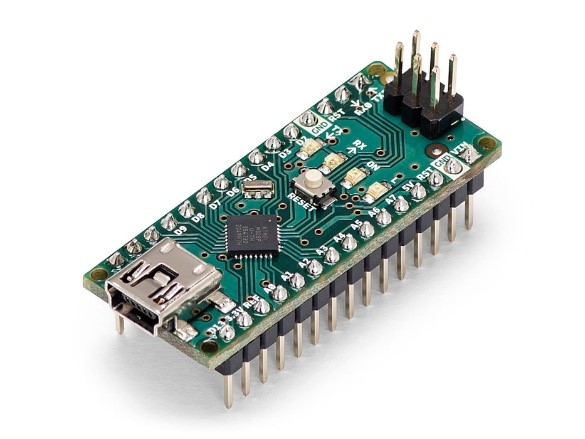
\includegraphics[width=0.8\textwidth]{2-1}
	\caption{Arduino Nano实物图}\label{fig:2-1}
\end{figure}

\begin{figure}[H]
	\centering
	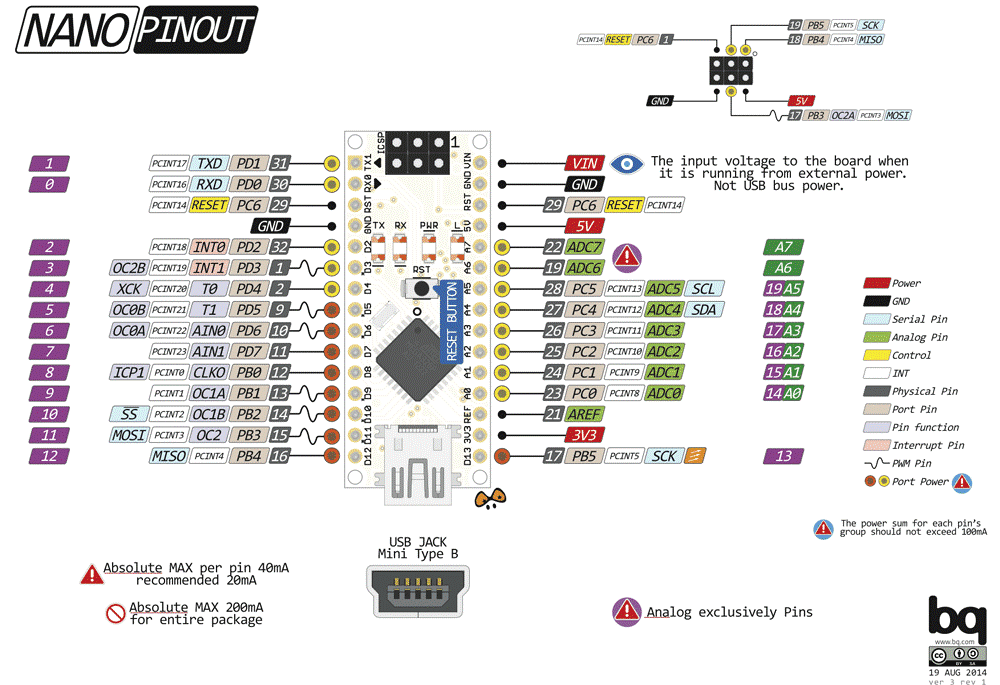
\includegraphics[width=0.9\textwidth]{2-2}
	\caption{引脚说明图}\label{fig:2-2}
\end{figure}

\subsection{SERVO42A闭环步进电机}

步进电机是通过脉冲信号来进行控制,每输入一个脉冲信号,步进电机前进一步。步进电机旋转的步距角,是在电机结构的基础上等比例控制产生的,如果控制电路的细分控制不变,那么步进旋转的步距角在理论上是一个固定的角度。这正好符号了魔方面旋转需要固定角度旋转的特性。


闭环步进电机与普通步进电机的区别在于闭环步进电机的闭环控制采用位置反馈或速度反馈~\cite{26}的方法来确定与转子位置相适应的相位转换~\cite{27},其目的是检测旋转的每一步是否都顺利完成,换言之是为了防止丢步。闭环电机如果出现丢步的情况,自身会通过反馈回电路的信息再补上,原用于生产精度要求比较高的3D打印机,考虑到其精度高,因此将其用于控制魔方面的旋转。

\begin{figure}[H]
	\centering
	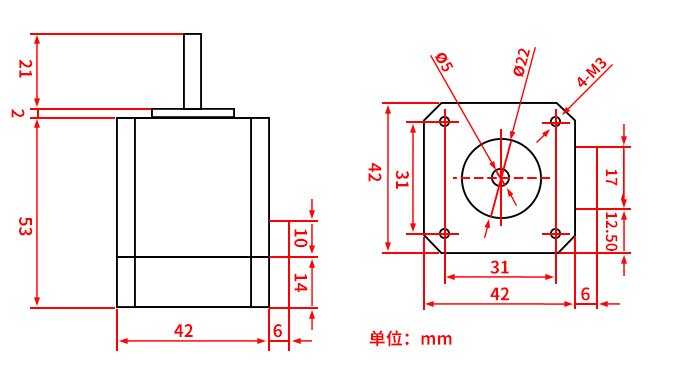
\includegraphics[width=0.5\textwidth]{2-3}
	\caption{SERVO42A电机尺寸图}\label{fig:2-3}
\end{figure}

\begin{figure}[H]
	\centering
	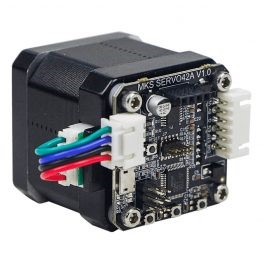
\includegraphics[width=0.5\textwidth]{2-4}
	\caption{SERVO42A电机实物图}\label{fig:2-4}
\end{figure}

闭环控制的步进电机系统或可在具有给定精确度下跟踪和反馈时,扩大工作速度范围,或可在给定速度下提高跟踪和定位精度,或可得到极限速度指标和极限精度指标。步进电机的闭环驱动很有意义,可实现完全无过冲的位置定位,在中低速应用中超越传统电机而取得一定的应用优势,最简单的闭环控制是在常规驱动器外加一个闭环控制器,使磁极磁通与电流的相位关系保持一致,产生能带动负载转矩的电磁转矩,除此之外,更加严格的闭环控制是以控制激磁磁通与电流相位角的方式对步进电机实施矢量控制,称作功率角闭环控制方法。不论哪种闭环控制方法,都可以大幅度提高顺滑性,降低功耗和固有震动。下表~\ref{tab:2-2}~是SERVO42A闭环步进电机的参数表。

\begin{table}[H]
	\caption{电机参数}\label{tab:2-2}
	\vspace{0.5em}
	\begin{center}
		{\wuhao
			\begin{tabular}{ccccc}
				\toprule
				属性 & 属性值	\\
				\midrule
				输入电压 & $12V-24V$\\
				峰值输出电流 & $\pm2A$\\
				闭环反馈频率 & $6kHz$\\
				精度 & $> 0.1125 ^{\circ} $\\
				细分步数 & $16,32,64,128,256$\\
				电机相数 & $2$\\
				保持转矩 & $\ge400mN \cdot m$\\
				转动惯量 & $62.5g \cdot cm^2$\\
				步距角 & $1.8^{\circ} \pm 5\% $ \\
				额定电流 & DC 1.0A/相\\
				\bottomrule
		\end{tabular}}
	\end{center}
	\vspace{-1.5em}
\end{table}

本系统选用闭环步进电机作为魔方一对一旋转的硬件部分,即一台闭环步进电机与一个魔方面相连接,同时,电机实现对魔方面的旋转控制意味着电机的旋转需要精确的位置控制。与开环步进电机相比,闭环步进电机最大的优势在于其高精度性,可稳定地进行旋转操作,具有更高的运行速度,更稳定、更光滑的转速。

\subsection{DS3120伺服电机}
伺服电机是一种传统的电机,在自动控制系统中用作执行元件。该电机可以控制速度,位置精度非常准确,可以将电压信号转化为转矩和转速以驱动控制对象。

伺服电机的转子转速受输入信号控制,并能快速反应,在自动控制系统中,用作执行元件,且具有机电时间常数小、线性度高等特性,可把所收到的电信号转换成电动机轴上的角位移或角速度输出。其主要作用是随着电压的变化控制转速均匀稳定。

伺服电机之所以精度非常准确,是因为靠脉冲来定位,当接受到一个脉冲电流,就会相应的旋转一个脉冲的对应角度,因为伺服电机本身也具有发出脉冲电流的功能,每当旋转一个角度都会发出对应数量的脉冲,和伺服电机接受的脉冲形成了呼应,或者叫闭环,因此能够精确的控制电机的转动,精确的定位可以达到0.001mm。

\begin{figure}[H]
	\centering
	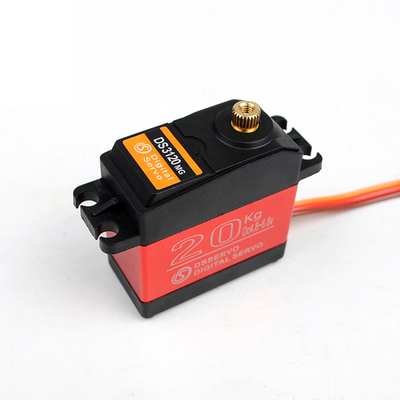
\includegraphics[width=0.4\textwidth]{2-5}
	\caption{伺服电机}\label{fig:2-5}
\end{figure}

与上一部分提到的闭环步进电机相比,伺服电机的精度更高,但是因为考虑到本系统需要同时考虑旋转速度,而伺服电机的旋转速度与闭环步进电机相差较大,因此并不能用于魔方面旋转。在本魔方还原系统中,伺服电机的作用在于将六个步进电机同时向位于中心的魔方移动,稳定魔方的位置,使其紧扣魔方中心块。


\section{六轴架构设计}
现有双臂解魔方机器人系统~\cite{10}~\cite{11}、四臂魔方还原系统~\cite{12}分别采用的是二轴、四轴的方式还原,而非六轴旋转还原的方式存在着单个旋转步骤需要分解为多个电机的旋转操作的缺点。两臂二指魔方机器人如下图~\ref{fig:2-6}~所示。

\begin{figure}[H]
	\centering
	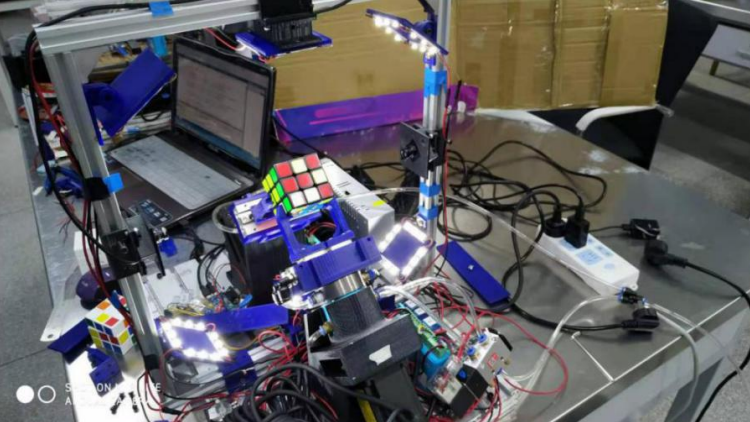
\includegraphics[width=0.8\textwidth]{2-6}
	\caption{两臂二轴魔方机器人}\label{fig:2-6}
\end{figure}

下图~\ref{fig:2-7}~是魔方建立三维坐标系后的示意图。以上述二轴魔方复原系统为例,假设该系统的两个旋转臂分别处于X轴正方向与Y轴正方向。此时若要还原魔方需要对Z轴正方向顺时针旋转 90° 。假设在二轴复原架构下,首先需要将X轴正方向的旋转臂顺时针旋转 90° ,将白色魔方面旋转至Y轴正方向,接着再将顺时针旋转Y轴正方向的旋转臂,两步操作后可复原魔方。但在本论文所设计的六轴复原架构下,只需要将位于Z轴正方向的电机顺时针旋转 90° 一步操作即可完成魔方复原。

也就是说,当需要旋转除与两臂直接接触的魔方面时,都需要进行额外的旋转操作,这将会大大增加魔方复原所消耗的时间,而这些冗余的时间也正是本论文提到的六轴复原架构所能节省的复原时间。

\begin{figure}[H]
	\centering
	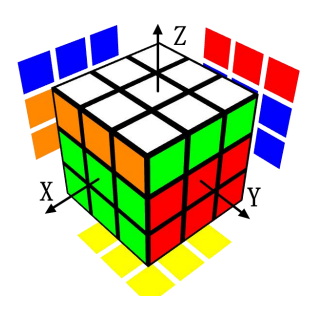
\includegraphics[width=0.55\textwidth]{2-7}
	\caption{带坐标轴的魔方示意图}\label{fig:2-7}
\end{figure}

六轴复原架构的具体实现方法是通过“爪子”将魔方中心块与电机一对一相连接,“爪子”与中心块的凹陷处紧扣后即可通过“爪子”的旋转带动魔方面的旋转。下列左图展示的是魔方中心块示意图,图中中心有四个小凹槽,分别与“爪子”四个凸起部分相匹配,右图是凹槽与“爪子”与红色魔方面相扣时的装配图。

\begin{figure}[H]
	\centering
	\subfigure{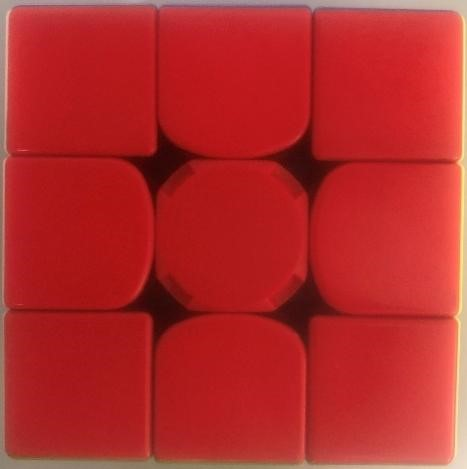
\includegraphics[height=5cm]{2-8}}
%	\hfill
	\subfigure{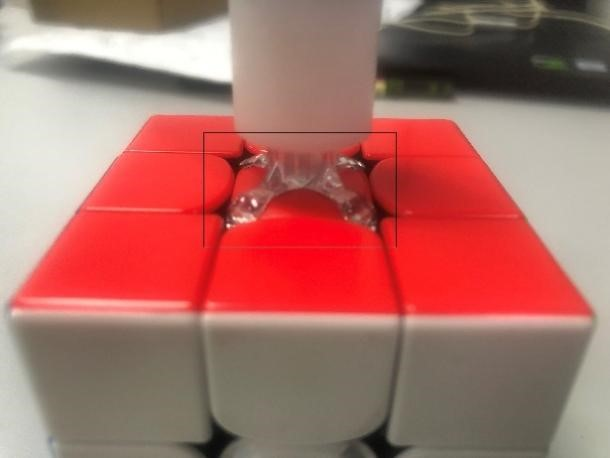
\includegraphics[height=5cm]{2-8.1}}
	\caption{魔方中心块示意图与装配图}\label{fig:2-8}
\end{figure}
本论文提出的六轴复原架构将魔方的六个面均采用上述“爪子”与魔方块一对一紧扣的方式相连接,该架构大大增加了系统的稳定性以及复原速度。

\section{PCB电路板设计}

为了使本魔方复原系统高度集成化,因此自主设计PCB电路板。

PCB电路板是将Arduino Nano下位机与闭环步进电机联结为一体的中间桥梁。该电路板外接12V适配器并搭配降压模块可同时分别向舵机提供5V电压,向步进电机提供12V电压。

此外,通过定义引脚以及电路板连线,将Arduino Nano发送旋转信号的引脚与相应电机的引脚相连接。电路板设计图与实物图如下图~\ref{fig:2-9}~所示,其中实物图左侧的蓝色模块为12V降压模块,可将12V电压降至5V电压,给舵机提供稳定5V电压。

\begin{figure}[H]
	\centering
	\subfigure[电路板设计图]{\label{fig:subfig:2-9}
		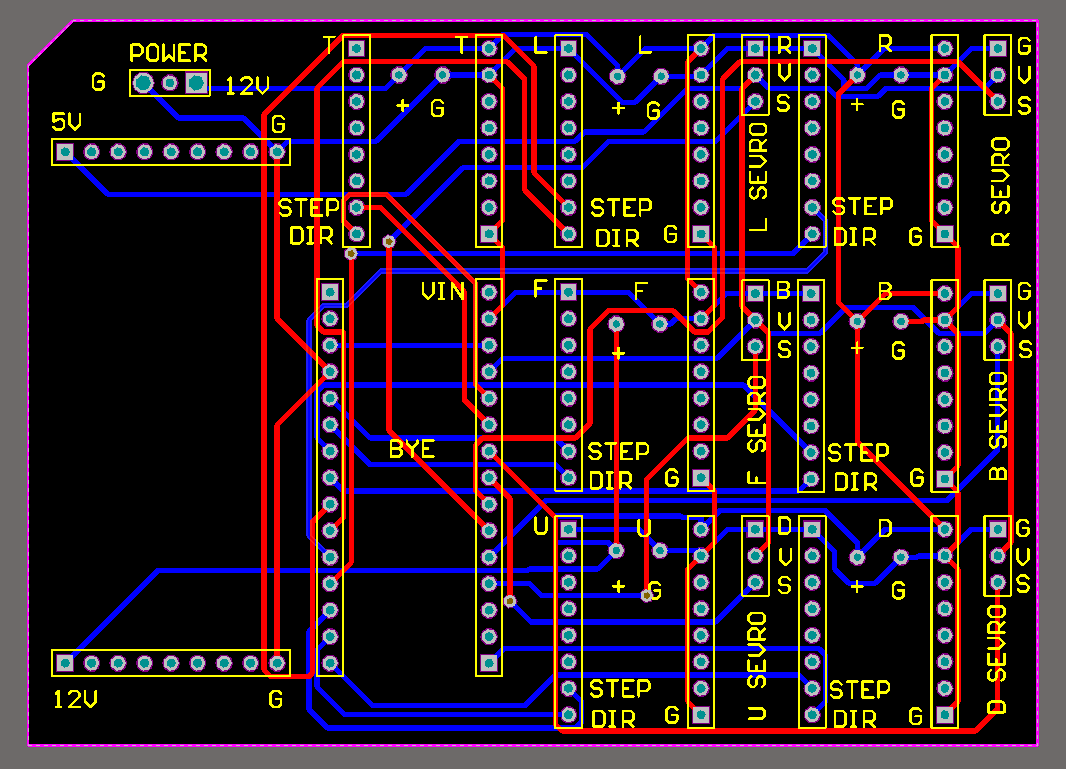
\includegraphics[height=5cm]{2-9}}
	\subfigure[电路板实物图]{\label{fig:subfig:2-9.1}
		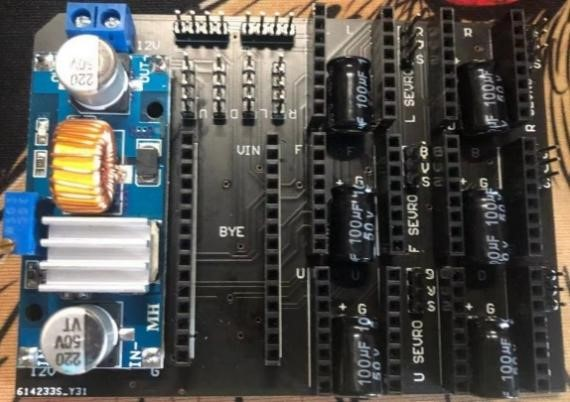
\includegraphics[height=5cm]{2-9.1}}
	\caption{电路板设计图与实物图}\label{fig:2-9}
\end{figure}

\section{三维建模结果图}

\subsection{零件仿真图}

本系统在三维建模阶段所用到的软件为SolidWorks2016,以下图~\ref{fig:2-10}~至图~\ref{fig:2-14}~为三维建模的仿真结果图。每个零件在系统中都有其独一无二、不可取代的作用。其中,图~\ref{fig:2-10}~所示的铝型材作为系统骨架,用于支撑整个系统;图~\ref{fig:2-11}~所示的滑轨用于平行移动步进电机,在伺服电机的驱动下可划动使其夹紧魔方;图~\ref{fig:2-12}~所示的滑块用于承载闭环其上方的步进电机,与图~\ref{fig:2-11}~的滑轨相配合;图~\ref{fig:2-13}~为步进电机与滑块的连接件,用于固定步进电机与滑块;图~\ref{fig:2-14}~为魔方托槽,用于放置本系统未运行状态时的魔方。

\begin{figure}[H]
	\centering
	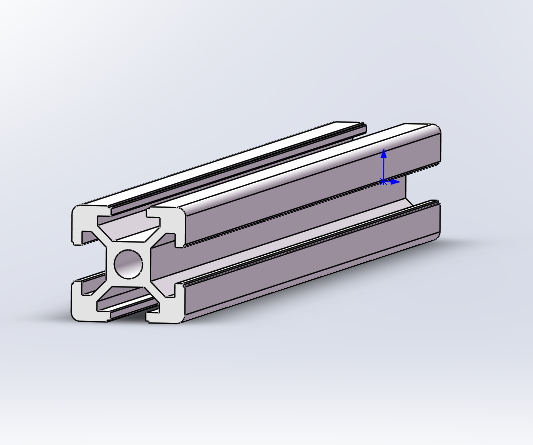
\includegraphics[width=0.6\textwidth]{2-10}
	\caption{铝型材仿真图}\label{fig:2-10}
\end{figure}

\begin{figure}[H]
	\centering
	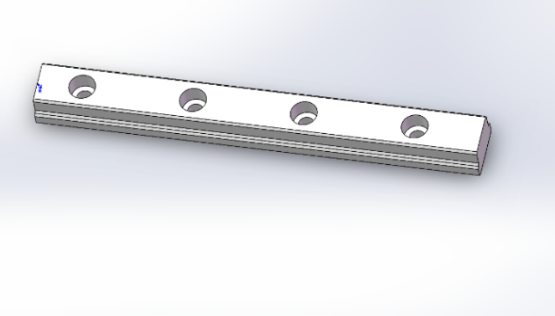
\includegraphics[width=0.6\textwidth]{2-11}
	\caption{滑轨仿真图}\label{fig:2-11}
\end{figure}

\begin{figure}[H]
	\centering
	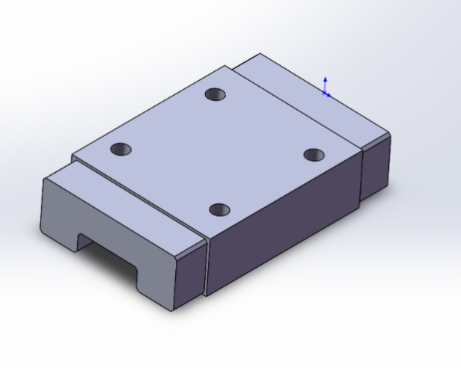
\includegraphics[width=0.6\textwidth]{2-12}
	\caption{滑块仿真图}\label{fig:2-12}
\end{figure}


\begin{figure}[H]
	\centering
	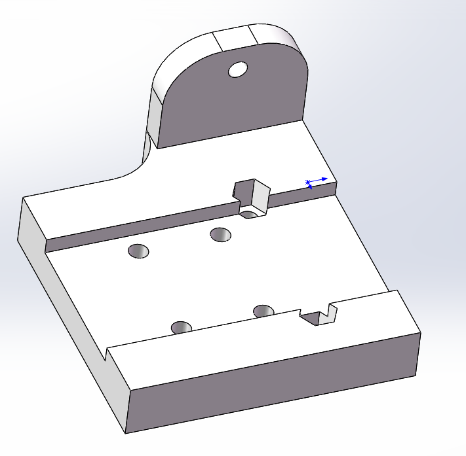
\includegraphics[width=0.6\textwidth]{2-13}
	\caption{电机滑块连接件仿真图}\label{fig:2-13}
\end{figure}


\begin{figure}[H]
\centering
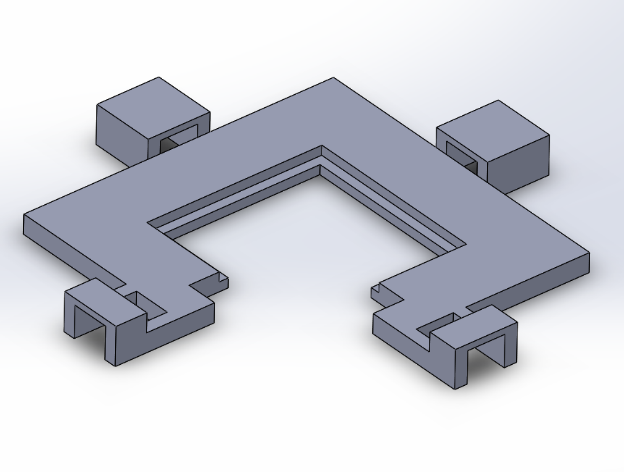
\includegraphics[width=0.6\textwidth]{2-14}
\caption{魔方托槽仿真图}\label{fig:2-14}
\end{figure}

\subsection{装配仿真图}

对于本论文提出的魔方复原系统,其装配结构对整体性能具有非常重要的影响。整个魔方还原系统需要设计多个方面的仿真结构,包括魔方与托槽装配仿真图、系统装配仿真图。

其中,下图~\ref{fig:2-15}~给出的魔方与托槽装配仿真图用于模拟仿真系统空闲时魔方放置在托槽上的状态;图~\ref{fig:2-16}~与图~\ref{fig:2-17}~的系统装配仿真图用于模拟仿真整个系统的硬件框架,在实际装配的过程中以该仿真图为参照物搭建整个系统,为整体系统搭建提供极大的便利。

\begin{figure}[H]
	\centering
	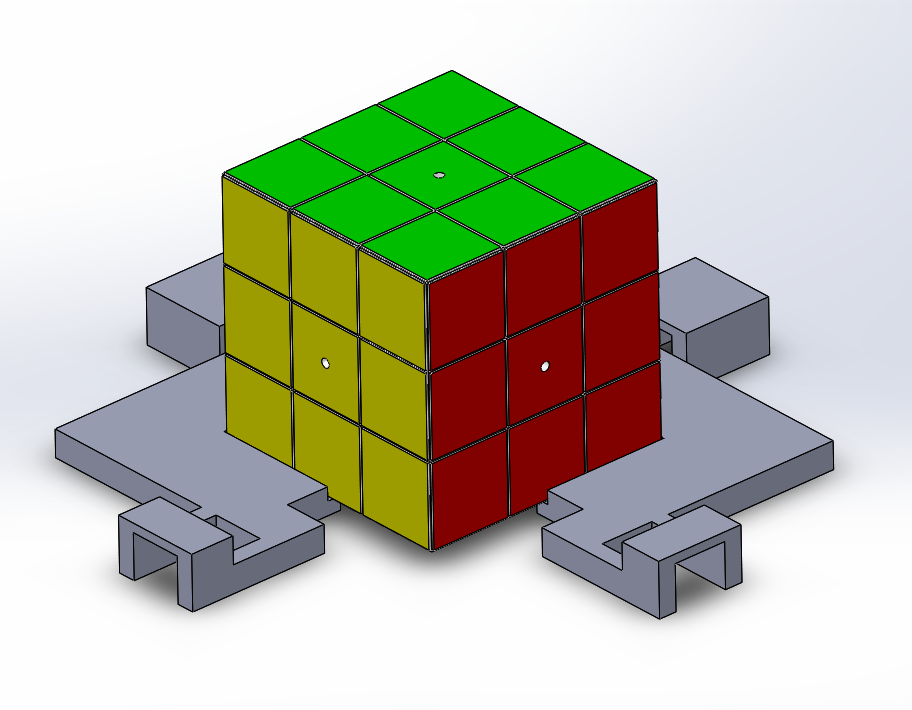
\includegraphics[width=0.6\textwidth]{2-15}
	\caption{魔方与托槽装配仿真图}\label{fig:2-15}
\end{figure}

\begin{figure}[H]
	\centering
	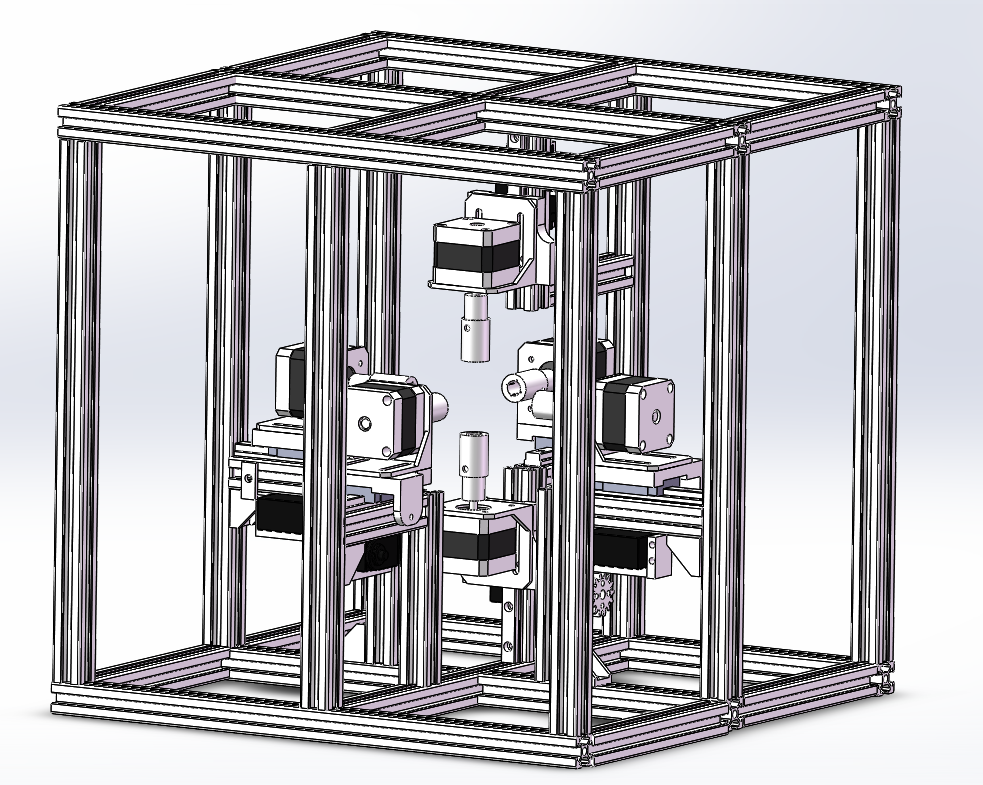
\includegraphics[width=0.6\textwidth]{2-16}
	\caption{系统装配仿真图(侧视图)}\label{fig:2-16}
\end{figure}

\begin{figure}[H]
	\centering
	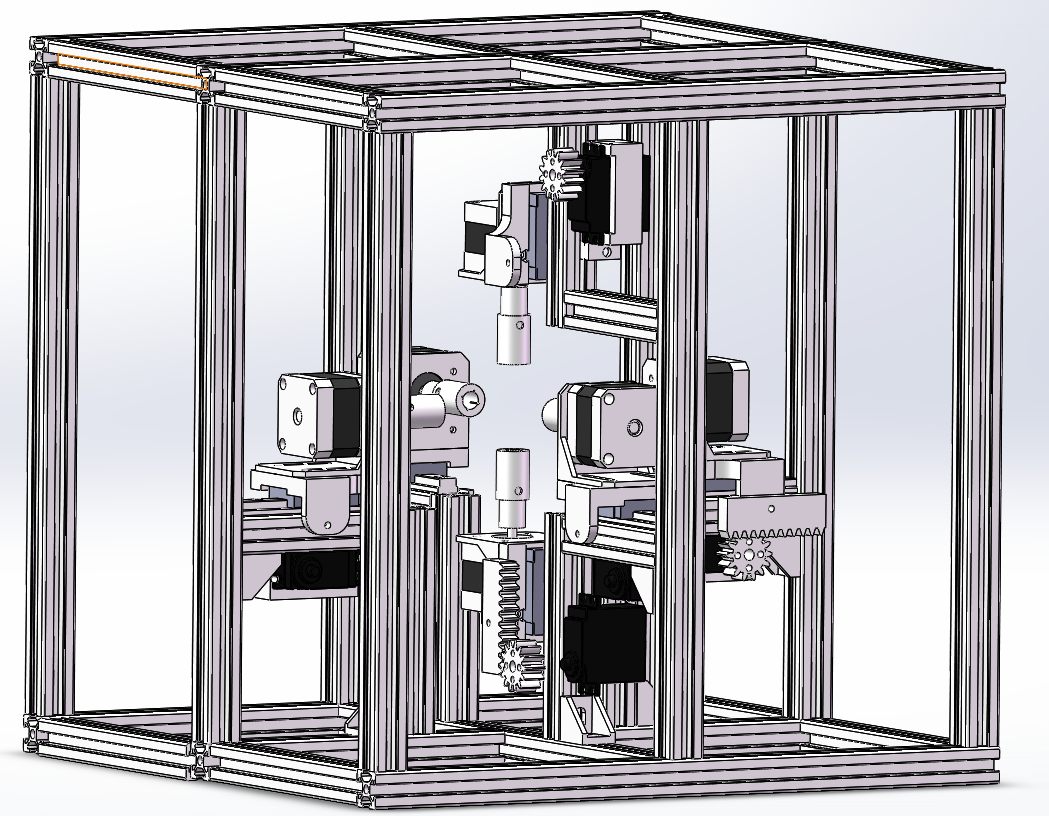
\includegraphics[width=0.6\textwidth]{2-17}
	\caption{系统装配仿真图(背视图)}\label{fig:2-17}
\end{figure}

\subsection{实际搭建效果图}

在本系统硬件部分的设计中,有一部分零件结合3D打印技术打印而成,也有一部分是使用现有相同规格的材料。图~\ref{fig:2-18}、图~\ref{fig:2-19}~为实际搭建的效果图,该框架是以上部分所示的仿真图为参照物进行系统搭建。

\begin{figure}[H]
	\centering
	\subfigure{
		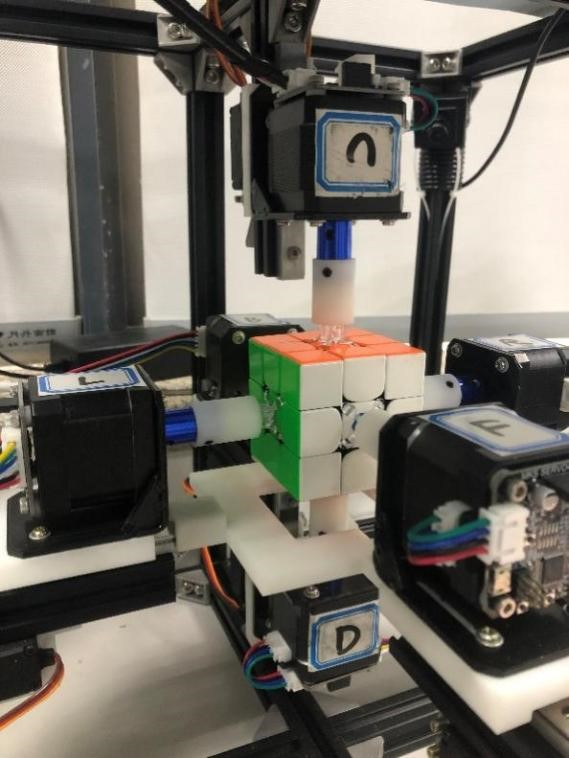
\includegraphics[width=0.4\textwidth]{2-18}}
	\subfigure{
		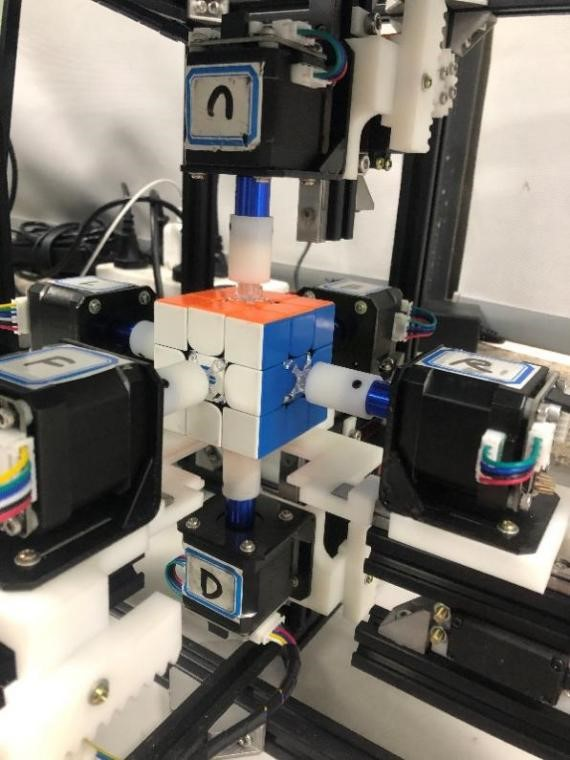
\includegraphics[width=0.4\textwidth]{2-18.1}}
	\caption{系统侧视图}\label{fig:2-18}
\end{figure}

\begin{figure}[H]
	\centering
	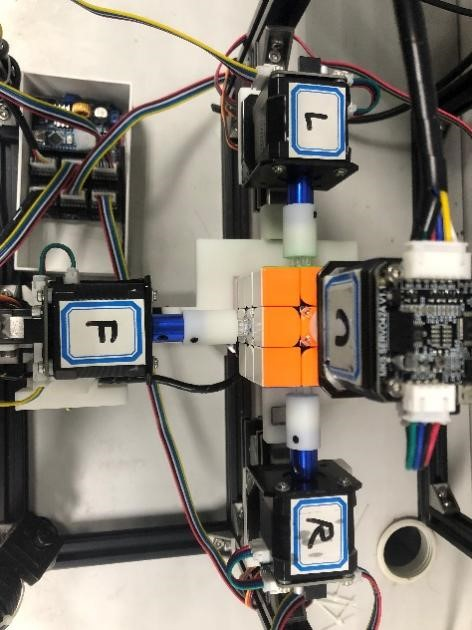
\includegraphics[angle=90,width=0.8\textwidth]{2-19}
	\caption{系统俯视图}\label{fig:2-19}
\end{figure}

\subsection{本章小结}

本章首先是介绍搭建本系统的硬件设备,接着简要阐述自主设计PCB电路板的思路,随后展示借助三维建模软件SolidWorks对魔方复原系统的框架整体搭建的建模结果图以及实际搭建后的效果图。本章列举本系统中硬件框架部分的内容,是本系统中最基础、最底层的一部分,为下一章系统软件算法的开发打下扎实的基础。
% !Mode:: "TeX:UTF-8"

\chapter{表格的绘制方法}

\section{本科生毕业设计论文的绘表规范}

表应有自明性。表格不加左、右边线。表的编排建议采用国际通行的三线表。表内中文书写使用宋体五号字。

每个表格之上均应有表题(由表序和表名组成)。表序一般按章编排,如第~1~章第一个插表的序号为“表~1-1”等。表序与表名之间空两格,
表名使用中文五号字,居中。表名中不允许使用标点符号,表名后不加标点。
表头设计应简单明了,尽量不用斜线。表头中可采用化学,物理量等专业符号。

全表如用同一单位,则将单位符号移至表头右上角,加圆括号。
表中数据应准确无误,书写清楚。数字空缺的格内加横线“-”(占~2~个数字宽度)。表内文字或数字上、下或左、右相同时,
采用通栏处理方式,不允许用“〃”、“同上”之类的写法。

表内文字使用宋体五号字,垂直居中书写,起行空一格、转行顶格、句末不加标点。
如某个表需要转页接排,在随后的各页上应重复表的编号。编号后加“(续表)”,表题可省略。续表应重复表头。
表格绘制完成之后,与正文空一行。

\section{普通表格的绘制方法}

表格应具有三线表格式,因此需要调用~booktabs~宏包,其标准格式如表~\ref{tab:table1}~所示。
\begin{table}[htbp]
\caption{符合本科生毕业论文绘图规范的表格}\label{tab:table1}
\vspace{0.5em}
\begin{center}
{\wuhao
\begin{tabular}{ccccc}
\toprule[1.5pt]
$D$(in) & $P_u$(lbs) & $u_u$(in) & $\beta$ & $G_f$(psi.in)\\
\midrule[1pt]
 5 & 269.8 & 0.000674 & 1.79 & 0.04089\\
10 & 421.0 & 0.001035 & 3.59 & 0.04089\\
20 & 640.2 & 0.001565 & 7.18 & 0.04089\\
 5 & 269.8 & 0.000674 & 1.79 & 0.04089\\
10 & 421.0 & 0.001035 & 3.59 & 0.04089\\
20 & 640.2 & 0.001565 & 7.18 & 0.04089\\
 5 & 269.8 & 0.000674 & 1.79 & 0.04089\\
10 & 421.0 & 0.001035 & 3.59 & 0.04089\\
20 & 640.2 & 0.001565 & 7.18 & 0.04089\\
 5 & 269.8 & 0.000674 & 1.79 & 0.04089\\
10 & 421.0 & 0.001035 & 3.59 & 0.04089\\
20 & 640.2 & 0.001565 & 7.18 & 0.04089\\
\bottomrule[1.5pt]
\end{tabular}}
\end{center}
\vspace{\baselineskip}
\end{table}

其绘制表格的代码及其说明如下。
\vspace{1em}\noindent\hrule

\begin{verbatim}
\begin{table}[htbp]
\caption{表标题}\label{标签名(通常为 tab:tablename)}
\vspace{0.5em}{\centering\wuhao
\begin{tabular}{cc...c}
\toprule[1.5pt]
表头第1个格   & 表头第2个格   & ... & 表头第n个格  \\
\midrule[1pt]
表中数据(1,1) & 表中数据(1,2) & ... & 表中数据(1,n)\\
表中数据(2,1) & 表中数据(2,2) & ... & 表中数据(2,n)\\
表中数据(3,1) & 表中数据(3,2) & ... & 表中数据(3,n)\\
表中数据(4,1) & 表中数据(4,2) & ... & 表中数据(4,n)\\
...................................................\\
表中数据(m,1) & 表中数据(m,2) & ... & 表中数据(m,n)\\
\bottomrule[1.5pt]
\end{tabular}}
\vspace{\baselineskip}
\end{table}
\end{verbatim}

\noindent\hrule

\begin{verbatim}
table环境是一个将表格嵌入文本的浮动环境。
\wuhao命令将表格的字号设置为五号字(10.5pt),在绘制表格结束退出时,不需要将字号再改回为\xiaosi,正文字号默认为小四号字(12pt)。 % XXX:重构之后不能这样做了,应该把整个表格用{\wuhao\begin{tabular}\ldots\end{tabular}} 包起来
tabular环境的必选参数由每列对应一个格式字符所组成:c表示居中,l表示左对齐,r表示右对齐,其总个数应与表的列数相同。此外,@{文本}可以出现在任意两个上述的列格式之间,其中的文本将被插入每一行的同一位置。表格的各行以\\分隔,同一行的各列则以&分隔。
\toprule、\midrule和\bottomrule三个命令是由booktabs宏包提供的,其中\toprule和\bottomrule分别用来绘制表格的第一条(表格最顶部)和第三条(表格最底部)水平线,\midrule用来绘制第二条(表头之下)水平线,且第一条和第三条水平线的线宽为1.5pt,第二条水平线的线宽为1pt。
引用方法:“如表~\ref{tab:tablename}~所示”。
\end{verbatim}

\noindent\hrule

\section{长表格的绘制方法}

长表格是当表格在当前页排不下而需要转页接排的情况下所采用的一种表格环境。若长表格仍按照普通表格的绘制方法来获得,
其所使用的~\verb|table|~浮动环境无法实现表格的换页接排功能,表格下方过长部分会排在表格第~1~页的页脚以下。为了能够实现长表格的转页接排功能,
需要调用~\verb|longtable|~宏包,由于长表格是跨页的文本内容,因此只需要单独的~\verb|longtable|~环境,所绘制的长表格的格式如表~\ref{tab:table2}~所示。

此长表格~\ref{tab:table2}~第~2~页的标题“编号(续表)”和表头是通过代码自动添加上去的,无需人工添加,若表格在页面中的竖直位置发生了变化,长表格在第~2~页
及之后各页的标题和表头位置能够始终处于各页的最顶部,也无需人工调整,\XeLaTeX~系统的这一优点是~Word~等软件所无法企及的。

下段内容是为了让下面的长表格分居两页,看到表标题“编号(续表)”的效果。此模板的完成时间正值雨后初霁的四月二十五日,故引用林徽因《你是人间的四月天》全文:
\begin{center}
\begin{minipage}[c]{0.5\textwidth}

\textbf{你是人间的四月天}

\vspace{12pt}
我说你是人间的四月天\\
笑音点亮了四面风\\
轻灵在春的光艳中交舞着变\\
你是四月早天里的云烟\\
黄昏吹着风的软\\
星子在无意中闪\\
细雨点洒在花前\\
那轻~~那娉婷\\
你是鲜妍\\
百花的冠冕你戴着\\
你是天真~~庄严~~你是夜夜的月圆\\
雪化后那片鹅黄\\
你像~~新鲜初放芽的绿\\
你是柔嫩喜悦\\
水光浮动着你梦期待中白莲\\
你是一树一树的花开\\
是燕~~在梁间呢喃\\
你是爱~~是暖\\
是希望\\
你是人间的四月天
\end{minipage}
\end{center}

{\wuhao{\begin{longtable}{cc}
\caption{浙江工业大学各学院名称一览}\label{tab:table2}
 \vspace{0.5em}\\
\toprule[1.5pt] 学院名称 & 网址\\ \midrule[1pt]
\endfirsthead
\multicolumn{2}{c}{表~\thetable(续表)}\vspace{0.5em}\\
\toprule[1.5pt] 学院名称 & 网址\\ \midrule[1pt]
\endhead
\bottomrule[1.5pt]
\endfoot
法学院 & \url{http://www.law.zjut.edu.cn/}\\
化学工程与材料学院 &  \url{http://www.ce.zjut.edu.cn/}\\
机械工程学院 & \url{http://www.jdxy.zjut.edu.cn/}\\
信息工程学院 & \url{http://www.ie.zjut.edu.cn/}\\
计算机科学与技术学院 & \url{http://www.software.zjut.edu.cn/}\\
软件学院 & \url{http://www.software.zjut.edu.cn/}\\
经贸管理学院 & \url{http://www.cba.zjut.edu.cn/}\\
建筑工程学院& \url{http://www.jgxy.zjut.edu.cn/}\\
生物与环境工程学院 & \url{http://www.bee.zjut.edu.cn/}\\
理学院 & \url{http://www.lxy.zjut.edu.cn/}\\
教育科学与技术学院 & \url{http://www.et.zjut.edu.cn/}\\
人文学院 & \url{http://www.rwxy.zjut.edu.cn/}\\
健行学院 & \url{http://www.jxxy.zjut.edu.cn/}\\
外国语学院 & \url{http://www.fl.zjut.edu.cn/}\\
国际学院 & \url{http://www.gjxy.zjut.edu.cn/}\\
政治与公共管理学院 & \url{http://www.sppa.zjut.edu.cn/}\\
艺术学院 & \url{http://www.art.zjut.edu.cn/}\\
药学院 & \url{http://www.yxy.zjut.edu.cn/}\\
成人教育学院 & \url{http://www.cj.zjut.edu.cn/}\\
之江学院 & \url{http://www.zjc.zjut.edu.cn/}\\
研究生院 & \url{http://www.gs.zjut.edu.cn/}\\
\end{longtable}}}
\vspace{\baselineskip}

绘制长表格的代码及其说明如下。
\vspace{1em}\noindent\hrule

\begin{verbatim}
{\wuhao\begin{longtable}{cc...c}
\caption{表标题}\label{标签名(通常为 tab:tablename)}\\
\toprule[1.5pt] 表头第1个格 & 表头第2个格 & ... & 表头第n个格\\ \midrule[1pt]
\endfirsthead
\multicolumn{n}{c}{表~\thetable(续表)}\vspace{0.5em}\\
\toprule[1.5pt] 表头第1个格 & 表头第2个格 & ... & 表头第n个格\\ \midrule[1pt]
\endhead
\bottomrule[1.5pt]
\endfoot
表中数据(1,1) & 表中数据(1,2) & ... & 表中数据(1,n)\\
表中数据(2,1) & 表中数据(2,2) & ... & 表中数据(2,n)\\
...................................................\\
表中数据(m,1) & 表中数据(m,2) & ... & 表中数据(m,n)\\
\end{longtable}}
\end{verbatim}

\noindent\hrule
\begin{verbatim}
在绘制长表格的前面留出一个空白行,并在第2行的一开始全局定义长表格的字号为五号字,这样能够保证长表格之前段落的行距保持不变。
在绘制长表格结束后,需要\xiaosi命令重新将字号改为小四号字。
\endhead之前的文字描述的是第2页及其之后各页的标题或表头;
\endfirsthead之前的文字描述的是第1页的标题和表头,若无此命令,则第1页的表头和标题由\endhead命令确定;
同理,\endfoot之前的文字描述的是除最后一页之外每页的表格底部内容;
\endlastfoot之前的文字描述的是最后一页的表格底部内容,若无此命令,
则最后一页的表格底部内容由\endfoot命令确定;由于规范中长表格每页底部内容均相同(水平粗线),因此模板中没有用到\endlastfoot命令。
\end{verbatim}

\noindent\hrule
\section{列宽可调表格的绘制方法}
论文中能用到列宽可调表格的情况共有两种:一种是当插入的表格某一单元格内容过长以至于一行放不下的情况,
另一种是当对公式中首次出现的物理量符号进行注释的情况。这两种情况都需要调用~tabularx~宏包。下面将分别对这两种情况下可调表格的绘制方法进行阐述。
\subsection{表格内某单元格内容过长的情况}

首先给出这种情况下的一个例子如表~\ref{tab:table3}~所示。
\begin{table}[htbp]
\caption{最小的三个正整数的英文表示法}\label{tab:table3}
\vspace{0.5em}{\wuhao
\begin{tabularx}{\textwidth}{llX}
\toprule[1.5pt]
Value & Name & Alternate names, and names for sets of the given size\\\midrule[1pt]
1 & One & ace, single, singleton, unary, unit, unity\\
2 & Two & binary, brace, couple, couplet, distich, deuce, double, doubleton, duad, duality, duet, duo, dyad, pair, snake eyes, span, twain, twosome, yoke\\
3 & Three & deuce-ace, leash, set, tercet, ternary, ternion, terzetto, threesome, tierce, trey, triad, trine, trinity, trio, triplet, troika, hat-trick\\\bottomrule[1.5pt]
\end{tabularx}}
\vspace{\baselineskip}
\end{table}
绘制这种表格的代码及其说明如下。
\vspace{1em}\noindent\hrule
\begin{verbatim}
\begin{table}[htbp]
\caption{表标题}\label{标签名(通常为 tab:tablename)}
\vspace{0.5em}{\wuhao
\begin{tabularx}{\textwidth}{l...X...l}
\toprule[1.5pt]
表头第1个格   & ... & 表头第X个格   & ... & 表头第n个格  \\
\midrule[1pt]
表中数据(1,1) & ... & 表中数据(1,X) & ... & 表中数据(1,n)\\
表中数据(2,1) & ... & 表中数据(2,X) & ... & 表中数据(2,n)\\
.........................................................\\
表中数据(m,1) & ... & 表中数据(m,X) & ... & 表中数据(m,n)\\
\bottomrule[1.5pt]
\end{tabularx}}
\vspace{\baselineskip}
\end{table}
\end{verbatim}

\noindent\hrule
\begin{verbatim}
tabularx环境共有两个必选参数:第1个参数用来确定表格的总宽度,这里取为排版表格能达到的最大宽度——正文宽度\textwidth;第2个参数用来确定每列格式,其中标为X的项表示该列的宽度可调,其宽度值由表格总宽度确定。
标为X的列一般选为单元格内容过长而无法置于一行的列,这样使得该列内容能够根据表格总宽度自动分行。若列格式中存在不止一个X项,则这些标为X的列的列宽相同,因此,一般不将内容较短的列设为X。
标为X的列均为左对齐,因此其余列一般选为l(左对齐),这样可使得表格美观,但也可以选为c或r。
\end{verbatim}

\noindent\hrule
\subsection{对物理量符号进行注释的情况}
为使得对公式中物理量符号注释的转行与破折号“———”后第一个字对齐,此处最好采用表格环境。此表格无任何线条,左对齐,
且在破折号处对齐,一共有“式中”二字、物理量符号和注释三列,表格的总宽度可选为文本宽度,因此应该采用\verb|tabularx|环境。
由\verb|tabularx|环境生成的对公式中物理量符号进行注释的公式如式(\ref{eq:1})所示。
%\vspace*{10pt}

\begin{equation}\label{eq:1}
\ddot{\boldsymbol{\rho}}-\frac{\mu}{R_{t}^{3}}\left(3\mathbf{R_{t}}\frac{\mathbf{R_{t}\rho}}{R_{t}^{2}}-\boldsymbol{\rho}\right)=\mathbf{a}
\end{equation}

\begin{tabularx}{\textwidth}{@{}l@{\quad}r@{———}X@{}}
式中& $\bm{\rho}$ &追踪飞行器与目标飞行器之间的相对位置矢量;\\
&  $\bm{\ddot{\rho}}$&追踪飞行器与目标飞行器之间的相对加速度;\\
&  $\mathbf{a}$   &推力所产生的加速度;\\
&  $\mathbf{R_t}$ & 目标飞行器在惯性坐标系中的位置矢量;\\
&  $\omega_{t}$ & 目标飞行器的轨道角速度;\\
&  $\mathbf{g}$ & 重力加速度,$=\frac{\mu}{R_{t}^{3}}\left(
3\mathbf{R_{t}}\frac{\mathbf{R_{t}\rho}}{R_{t}^{2}}-\bm{\rho}\right)=\omega_{t}^{2}\frac{R_{t}}{p}\left(
3\mathbf{R_{t}}\frac{\mathbf{R_{t}\rho}}{R_{t}^{2}}-\bm{\rho}\right)$,这里~$p$~是目标飞行器的轨道半通径。
\end{tabularx}
\vspace{\wordsep}

其中生成注释部分的代码及其说明如下。

\vspace{1em}\noindent\hrule

\begin{verbatim}
\begin{tabularx}{\textwidth}{@{}l@{\quad}r@{— — —}X@{}}
式中 & symbol-1 & symbol-1的注释内容;\\
     & symbol-2 & symbol-2的注释内容;\\
     .............................;\\
     & symbol-m & symbol-m的注释内容。
\end{tabularx}\vspace{\wordsep}
\end{verbatim}

\noindent\hrule\vspace{1em}

%\begin{verbatim}
   tabularx环境的第1个参数选为正文宽度,第2个参数里面各个符号的意义为:
   第1个@{}表示在“式中”二字左侧不插入任何文本,“式中”二字能够在正文中左对齐,若无此项,则“式中”二字左侧会留出一定的空白;
   @{\quad}表示在“式中”和物理量符号间插入一个空铅宽度的空白;
   @{— — —}实现插入破折号的功能,它由三个1/2的中文破折号构成;
   第2个@{}表示在注释内容靠近正文右边界的地方能够实现右对齐。
%\end{verbatim}
\vspace{1em}
\noindent\hrule\vspace{1em}

由此方法生成的注释内容应紧邻待注释公式并置于其下方,因此不能将代码放入~\verb|table|~浮动环境中。但此方法不能实现自动转页接排,
可能会在当前页剩余空间不够时,全部移动到下一页而导致当前页出现很大空白。因此在需要转页处理时,还请您手动将需要转页的代码放入一个
新的~\verb|tabularx|~环境中,将原来的一个~\verb|tabularx|~环境拆分为两个~\verb|tabularx|~环境。

若想获得绘制表格的更多信息,参见网络上的~\href{http://www.tug.org/pracjourn/2007-1/mori/}{Tables in \LaTeXe: Packages and Methods}~文档。


% !Mode:: "TeX:UTF-8"

\chapter{数学公式的输入方法}
\section{本科生毕业设计论文的公式规范}

论文中的公式应另起行,原则上应居中书写,与周围文字留有足够的空间区分开。
若公式前有文字(如“解”、“假定”等),文字空两格写,公式仍居中写。公式末不加标点。

公式应标注序号,并将序号置于括号内。 公式序号按章编排,如第~1~章第一个公式序号为“(1-1)”。公式的序号右端对齐。

公式较长时最好在等号“=”处转行,如难实现,则可在~$+$、$-$、$\times$、$\div$~运算符号处转行,转行时运算符号仅书写于转行式前,不重复书写。

文中引用公式时,一般用“见式~(1-1)”或“由公式~(1-1)”。

公式中用斜线表示“除”的关系时应采用括号,以免含糊不清,如~$a/(b\cos x)$。通常“乘”的关系在前,如~$a\cos x/b$而不写成~$(a/b)\cos x$。

不能用文字形式表示等式,如:$\textnormal{刚度}=\frac{{\textnormal{受力}}}{{\textnormal{受力方向的位移}}}$。

对于数学公式的输入方法,网络上有一个比较全面权威的文档\textbf{~\href{http://tug.ctan.org/cgi-bin/ctanPackageInformation.py?id=voss-mathmode}{Math mode}}~请大家事先大概浏览一下。下面将对学位论文中主要用到的数学公式排版形式进行阐述。

\section{生成~\XeLaTeX~数学公式的两种方法}
对于先前没有接触过~\XeLaTeX~的人来说,编写~\XeLaTeX~数学公式是一件很繁琐的事,尤其是对复杂的数学公式来说,更可以说是一件难以完成的任务。
实际上,生成~\XeLaTeX~数学公式有两种较为简便的方法,一种是基于~MathType~数学公式编辑器的方法,另一种是基于~MATLAB~商业数学软件的方法,
下面将分别对这两种数学公式的生成方法作一下简单介绍。

\subsection{基于~MathType~软件的数学公式生成方法}
MathType~是一款功能强大的数学公式编辑器软件,能够用来在文本环境中插入~Windows OLE~图形格式的复杂数学公式,所以应用比较普遍。但此软件只有~30~天的试用期,之后若再继续使用则需要付费购买才行。网络上有很多破解版的~MathType~软件可供下载免费使用,
笔者推荐下载安装版本号在~6.5~之上的中文破解版。

在安装好~MathType~之后,若在输入窗口中编写数学公式,复制到剪贴板上的仍然是图形格式的对象。
若希望得到可插入到~\XeLaTeX~编辑器中的文本格式对象,则需要对~MathType~软件做一下简单的设置:在~MathType~最上排的按钮中依次选择“参数选项
$\to$转换”,在弹出的对话窗中选中“转换到其它语言(文字):”,在转换下拉框中选择“Tex~--~--~LaTeX 2.09 and later”,并将对话框最下方的两个复选框全部勾掉,点击确定,这样,再从输入窗口中复制出来的对象就是文本格式的了,就可以直接将其粘贴到~\XeLaTeX~
编辑器中了。按照这种方法生成的数学公式两端分别有标记\verb|\[|和标记\verb|\]|,在这两个标记之间才是真正的数学公式代码。

若希望从~MathType~输入窗口中复制出来的对象为图形格式,则只需再选中“公示对象(Windows OLE~图形)”即可。

\subsection{基于~MATLAB~软件的数学公式生成方法}

MATLAB~是矩阵实验室(Matrix Laboratory)的简称,是美国~MathWorks~公司出品的商业数学软件。它是当今科研领域最常用的应用软件之一,
具有强大的矩阵计算、符号运算和数据可视化功能,是一种简单易用、可扩展的系统开发环境和平台。

MATLAB~中提供了一个~latex~函数,它可将符号表达式转化为~\XeLaTeX~数学公式的形式。其语法形式为~latex(s),其中,~s~为符号表达式,
之后再将~latex~函数的运算结果直接粘贴到~\XeLaTeX~编辑器中。从~\XeLaTeX~数学公式中可以发现,其中可能包含如下符号组合:

\begin{verbatim*}
\qquad=两个空铅(quad)宽度
\quad=一个空铅宽度
\;=5/18空铅宽度
\:=4/18空铅宽度
\,=3/18空铅宽度
\!=-3/18空铅宽度
\ =一个空格
\end{verbatim*}

所以最好将上述符号组合从数学公式中删除,从而使数学公式显得匀称美观。

对于~Word~等软件的使用者来说,在我们通过~MATLAB~运算得到符号表达式形式的运算结果时,在~Word~中插入运算结果需要借助于~MathType~软件,
通过在~MathType~中输入和~MATLAB~运算结果相对应的数学表达形式,之后再将~MathType~数学表达式转换为图形格式粘贴到~Word~中。实际上,
也可以将~MATLAB~中采用~latex~函数运行的结果直接粘贴到~MathType~中,再继续上述步骤,这样可以大大节省输入公式所需要的时间。
此方法在~MathType~6.5c~上验证通过,若您粘入到~MathType~中的仍然为从~MATLAB~中导入的代码,请您更新~MathType~软件。

\section{数学字体}
在数学模式下,常用的数学字体命令有如下几种:

\begin{verbatim}
\mathnormal或无命令 用数学字体打印文本;
\mathit             用斜体(\itshape)打印文本;
\mathbf             用粗体(\bfseries)打印文本;
\mathrm             用罗马体(\rmfamily)打印文本;
\mathsf             用无衬线字体(\sffamily)打印文本;
\mathtt             用打印机字体(\ttfamily)打印文本;
\mathcal            用书写体打印文本;
\end{verbatim}

在学位论文撰写中,只需要用到上面提到的~\verb|\mathit|、\verb|\mathbf|~和~\verb|\mathrm|~命令。若要得到~Times New Roman~的数学字体,则需要调用~txfonts~宏包(此宏包实际上采用的是~Nimbus Roman No9 L~字体,
它是开源系统中使用的免费字体,其字符字体与~Times New Roman~字体几乎完全相同);若要得到粗体数学字体,则需要调用~bm~宏包。表~\ref{tab:fonts}~中分别列出了得到阿拉伯数字、拉丁字母和希腊字母
各种数学字体的命令。

\begin{table}[htbp]
\caption{常用数学字体命令一览}\label{tab:fonts}
\vspace{0.5em}\centering\wuhao
\begin{tabular}{llll}
\toprule
 & 阿拉伯数字\&大写希腊字母 & 大小写拉丁字母 & 小写希腊字母  \\
\midrule
斜体 & \verb|\mathit{}| & \verb|无命令| & \verb|无命令|\\
粗斜体 & \verb|\bm{\mathit{}}| & \verb|\bm{}| & \verb|\bm{}|\\
直立体 & \verb|无命令| & \verb|\mathrm{}| & \verb|字母后加up|\\
粗体 & \verb|\mathbf{}或\bm{}| & \verb|\mathbf{}| & \verb|\bm{字母后加up}|\\
\bottomrule
\end{tabular}
\vspace{\baselineskip}
\end{table}

\noindent 下面列出了一些应采用直立数学字体的数学常数和数学符号。

\section{行内公式}
出现在正文一行之内的公式称为行内公式,例如~$f(x)=\int_{a}^{b}\frac{\sin{x}}{x}dx$。对于非矩阵和非多行形式的行内公式,一般不会使得行距发生变化,而~Word~等软件却会根据行内公式的竖直距离而自动调节行距,如图~\ref{fig:hangju}~所示。

\begin{figure}[htbp]
\centering
\subfigure[由~\XeLaTeX~系统生成的行内公式]{\label{fig:subfig:latex}
                \fbox{\includegraphics[width=0.55\textwidth]{latex}}}
\subfigure[由~Word软件生成的~.doc~格式行内公式]{\label{fig:subfig:word}
                \fbox{\includegraphics[width=0.55\textwidth]{word}}}
\subfigure[由~Word软件生成的~.pdf~格式行内公式]{\label{fig:subfig:pdf}
                \fbox{\includegraphics[width=0.55\textwidth]{pdf}}}

\caption{由~\XeLaTeX~和~Word~生成的~3~种行内公式屏显效果}\label{fig:hangju}
\vspace{-1em}
\end{figure}

这三幅图分别为~\XeLaTeX~和~Word~生成的行内公式屏显效果,从图中可看出,在~\XeLaTeX~文本含有公式的行内,在正文与公式之间对接工整,行距不变;而在~Word~文本含有公式的行内,在正文与公式之间对接不齐,行距变大。因此从这一点来说,
\XeLaTeX~系统在数学公式的排版上具有很大优势。

\XeLaTeX~提供的行内公式最简单、最有效的方法是采用~\TeX~本来的标记———开始和结束标记都写作~\$,例如本段开始的例子可由下面的输入得到。
\verb|$f(x)=\int_{a}^{b}\frac{\sin{x}}{x}\mathrm{d}x$|

\section{行间公式}
位于两行之间的公式称为行间公式,每个公式都是一个单独的段落,例如
\[\int_a^b{f\left(x\right)\mathrm{d}x}=\lim_{\left\|\Delta{x_i}\right\|\to 0}\sum_i{f\left(\xi_i\right)\Delta{x_i}}\]
除人工编号外,\XeLaTeX~无编号行间公式的标记见表~\ref{tab:eqtag_1},自动编号行间公式的标记间表~\ref{tab:eqtag_2}。
\begin{table}[htbp]
\caption{无编号行间公式的标记}\label{tab:eqtag_1}
\vspace{0.5em}\centering\wuhao
\begin{tabularx}{\textwidth}{cc}
\toprule
& 无编号\\
\midrule
单行公式 & \verb|\begin{displaymath}... \end{displaymath}| 或~\verb|\[...\]|\\
多行公式 & \verb|\begin{eqnarray*}... \end{eqnarray*}|\\
\bottomrule
\end{tabularx}
\end{table}

\begin{table}[htbp]
\caption{自动编号行间公式的标记}\label{tab:eqtag_2}
\vspace{0.5em}\centering\wuhao
\begin{tabularx}{\textwidth}{cc}
\toprule
& 自动编号\\
\midrule
单行公式 & \verb|\begin{equation}... \end{equation}|\\
多行公式 & \verb|\begin{eqnarray}... \end{eqnarray}|\\
\bottomrule
\end{tabularx}
\end{table}

另外,在自动编号的某行公式行尾添加标签~\verb|\nonumber|,可将该行转换为无编号形式。

行间多行公式需采用~\verb|eqnarray|~或~\verb|eqnarray*|~环境,它默认是一个列格式为~\verb|rcl|~的~3~列矩阵,并且中间列的字号要小一些,因此通常只将需要对齐的运算符号(通常为等号“=”)置于中间列。

\section{常见的数学式}
本节列举一些常见的数学式作为练习与未来使用的参考,每个函数都有其特别之处,请仔细观察研究。
读者可以依此为基础,在往后的写作过程中,逐渐累积更多有特殊型态的或符号的数学式,
只要这里出现过的,参照原使档一定写得出来。

\subsection{函数}
\begin{lstlisting}[language=TeX,numbers=none,frame=lrtb,keywords={begin},label=Binomial,caption=Binomial] 
$f(x)={n\choose x}p^x(1-p)^{1-x}, \;\; x=0,1,2,\cdots,n$ 
\end{lstlisting}
$f(x)={n\choose x}p^x(1-p)^{1-x}, \;\; x=0,1,2,\cdots,n$ 
   
\begin{lstlisting}[language=TeX,numbers=none,frame=lrtb,keywords={begin},label=Poisson,caption=Poisson] 
$f(x)=\frac{e^{-\lambda}\lambda^x}{x!}, \;\;  x=0,1,2,\cdots$ 
\end{lstlisting}
$f(x)=\frac{e^{-\lambda}\lambda^x}{x!}, \;\;  x=0,1,2,\cdots$
  
\begin{lstlisting}[language=TeX,numbers=none,frame=lrtb,keywords={begin},label=Gamma,caption=Gamma] 
$f(x)=\frac{1}{\Gamma(\alpha)\beta^\alpha}x^{\alpha-1} e^{-\frac{x}{\beta}}, \;\; x\geq 0$
\end{lstlisting}
$f(x)=\frac{1}{\Gamma(\alpha)\beta^\alpha}x^{\alpha-1}e^{-\frac{x}{\beta}}, \;\; x\geq 0$ 
  
\begin{lstlisting}[language=TeX,numbers=none,frame=lrtb,keywords={begin},label=Normal,caption=Normal] 
$f(x)=\frac{1}{\sigma\sqrt{2\pi}}e^{-\frac{(x-\mu)^2}{2\sigma^2}}, \;\;  -\infty < x < \infty $
\end{lstlisting}
$f(x)=\frac{1}{\sigma\sqrt{2\pi}}e^{-\frac{(x-\mu)^2}{2\sigma^2}}, \;\;  -\infty < x < \infty $
  
\begin{lstlisting}[language=TeX,numbers=none,frame=lrtb,keywords={begin},label=Int,caption=积分式与方程式编号] 
\begin{equation}\label{gamma}%..........label后的名称自订,代表该方程式
\int^\infty_0 x^{\alpha-1}e^{-\lambda x} dx = \frac{\Gamma(\alpha)}{\lambda^{\alpha}}
\end{equation}
\end{lstlisting}
\begin{equation}\label{gamma}%.................label后的名称自订,代表该方程式
\int^\infty_0 x^{\alpha-1}e^{-\lambda x} dx = \frac{\Gamma(\alpha)}{\lambda^{\alpha}}
\end{equation}
  
方程式 (\ref{gamma})是广义 $\Gamma$ 积分。\footnote{这里利用方程式标签(label)来引用方程式,编号将自动更新。}
 
\begin{lstlisting}[language=TeX,numbers=none,frame=lrtb,keywords={begin},label=Sqrt,caption=开根号] 
$$f(x)=\sqrt[3]{\frac {\displaystyle 4-x^{3}}{\displaystyle 1+x^{2}}}$$
\end{lstlisting}
$$f(x)=\sqrt[3]{\frac {\displaystyle 4-x^{3}}{\displaystyle 1+x^{2}}}$$
  
\begin{lstlisting}[language=TeX,numbers=none,frame=lrtb,keywords={begin},label=limit,caption=微分与极限(注意大刮号的使用)] 
$$f'(x)=\frac{df(x)}{dx}=\lim_{h\rightarrow 0} \left( \frac{f(x+h)-f(x)}{h} \right)$$
\end{lstlisting}  
$$f'(x)=\frac{df(x)}{dx}=\lim_{h\rightarrow 0}\left(\frac{f(x+h)-f(x)}{h}\right)$$

\begin{lstlisting}[language=TeX,numbers=none,frame=lrtb,keywords={begin},label=upanddown,caption=上下限的使用] 
$$\int_a^b f(x) dx \approx \lim_{n\rightarrow \infty}\sum_{k=1}^n f(x_k)\triangle x_k$$
\end{lstlisting} 
$$\int_a^b f(x) dx \approx \lim_{n\rightarrow \infty}\sum_{k=1}^n f(x_k)\triangle x_k$$
  
\begin{lstlisting}[language=TeX,numbers=none,frame=lrtb,keywords={begin},label=bast,caption=最佳化问题] 
$$\max_{\mathbf{u},\mathbf{u}^T\mathbf{u}=1} \mathbf{u}^T\Sigma_X\mathbf{u}$$
\end{lstlisting} 
$$\max_{\mathbf{u},\mathbf{u}^T\mathbf{u}=1} \mathbf{u}^T\Sigma_X\mathbf{u}$$
  
\begin{lstlisting}[language=TeX,numbers=none,frame=lrtb,keywords={begin},label=somesymbles,caption=几个符号]
$$\mathbf{e}=\mathbf{x}-\mathbf{x}_q=(I-P)\mathbf{x} \in V^{\perp}, \mbox{where}\; V\oplus V^{\perp}=R^p $$
\end{lstlisting} 
$$\mathbf{e}=\mathbf{x}-\mathbf{x}_q=(I-P)\mathbf{x} \in V^{\perp}, \mbox{where}\; V\oplus V^{\perp}=R^p $$


\subsection{矩阵与行列式}
矩阵或有规则排列的数学式或组合很常见,以下列举几种模式,请特别注意其使用的标签及一些需要注意的小地方。譬如,
\begin{enumerate}%[a)]
\item 矩阵的左右括号需各别加上。
\item 横行各项之间是以 $\&$ 区隔。
\item 除最后一行外,每行之末则加上换行指令$\backslash$ $\backslash$。
\item 使用array指令时,须加上选项以控制每一直栏内各数字或符号要居中排列、靠左或靠右。
\end{enumerate}
范例与注意事项:
\begin{enumerate}
  \item 左右方框刮号的使用及各直栏的对齐方式:
        $$ A = \left[
            \begin{array}{clr}
                a+b & mnop  & xy \\
                a+b & pn    & yz \\
                b+c & mp    & xyz
            \end{array} \right] $$
\begin{lstlisting}[language=TeX,numbers=none,frame=lrtb,keywords={begin}]
$$ A = \left[
\begin{array}{clr}
a+b & mnop  & xy \\
a+b & pn    & yz \\
b+c & mp    & xyz
\end{array} \right] $$
\end{lstlisting} 

\item 左右圆框刮号的使用及各式点状:
$$ A=\left(
\begin{array}{cccc}
a_{11} & a_{12} & \cdots & a_{1n}\\
a_{21} & a_{22} & \cdots & a_{2n}\\
\vdots & \vdots & \ddots & \vdots\\
a_{n1} & a_{n2} & \cdots & a_{nn}
\end{array} \right) $$
\begin{lstlisting}[language=TeX,numbers=none,frame=lrtb,keywords={begin}]
$$ A=\left(
\begin{array}{cccc}
a_{11} & a_{12} & \cdots & a_{1n}\\
a_{21} & a_{22} & \cdots & a_{2n}\\
\vdots & \vdots & \ddots & \vdots\\
a_{n1} & a_{n2} & \cdots & a_{nn}
\end{array} \right) $$
\end{lstlisting} 

\item 排列整齐的符号:
$$ \begin{array}{clr}\\
a+b+c   & m+n & xy \\
a+b     & p+n & yz \\
b+c     & m-n & xz
\end{array} $$
\begin{lstlisting}[language=TeX,numbers=none,frame=lrtb,keywords={begin}]
$$ \begin{array}{clr}\\
a+b+c   & m+n & xy \\
a+b     & p+n & yz \\
b+c     & m-n & xz
\end{array} $$
\end{lstlisting}

\item 等号对齐的函数组合(不编号)
\begin{eqnarray*}
b_1 &=& d_1+c_1 \\
a_2 &=& c_2+e_2
\end{eqnarray*}
\begin{lstlisting}[language=TeX,numbers=none,frame=lrtb,keywords={begin}]
\begin{eqnarray*}
b_1 &=& d_1+c_1 \\
a_2 &=& c_2+e_2
\end{eqnarray*}
\end{lstlisting}

\item 等号对齐的函数组合(编号在最后一行)
\begin{eqnarray}
\nonumber b_1 &=& d_1+c_1 \\
a_2 &=& c_2+e_2
\end{eqnarray}
\begin{lstlisting}[language=TeX,numbers=none,frame=lrtb,keywords={begin}]
\begin{eqnarray}
\nonumber b_1 &=& d_1+c_1 \\
a_2 &=& c_2+e_2
\end{eqnarray}
\end{lstlisting}

\item 使用巨集 amsmath 的指令 align(控制编号在第一行)
\begin{align}
b_1 &= d_1+c_1\\
a_2 &= c_2+e_2 \notag
\end{align}
\begin{lstlisting}[language=TeX,numbers=none,frame=lrtb,keywords={begin}]
\begin{align}
b_1 &= d_1+c_1\\
a_2 &= c_2+e_2 \notag
\end{align}
\end{lstlisting}

\item 两组数学式分别对齐
\begin{align}
\alpha_1 &= \beta_1+\gamma_1+\delta_1, &a_1 &= b_1+c_1\\
\alpha_2 &= \beta_2+\gamma_2+\delta_2, &a_2 &= b_2+c_2
\end{align}
\begin{lstlisting}[language=TeX,numbers=none,frame=lrtb,keywords={begin}]
\begin{align}
\alpha_1 &= \beta_1+\gamma_1+\delta_1, &a_1 &= b_1+c_1\\
\alpha_2 &= \beta_2+\gamma_2+\delta_2, &a_2 &= b_2+c_2
\end{align}
\end{lstlisting}

\item 编号在中间(split指令环境)
\begin{equation}
\begin{split}
\alpha_1 &= \beta_1+\gamma_1\\
\alpha_2 &= \beta_2+\gamma_2
\end{split}
\end{equation}
\begin{lstlisting}[language=TeX,numbers=none,frame=lrtb,keywords={begin}]
\begin{equation}
\begin{split}
\alpha_1 &= \beta_1+\gamma_1\\
\alpha_2 &= \beta_2+\gamma_2
\end{split}
\end{equation}
\end{lstlisting}

\item 只是居中对齐的数学式组(gather指令环境)
\begin{gather}
\alpha_1 + \beta_1\notag\\
\alpha_2 + \beta_2 + \gamma_2\notag
\end{gather}
\begin{lstlisting}[language=TeX,numbers=none,frame=lrtb,keywords={begin}]
\begin{gather}
\alpha_1 + \beta_1\notag\\
\alpha_2 + \beta_2 + \gamma_2\notag
\end{gather}
\end{lstlisting}

\item 长数学式的表达(注意第二行加号的位置)
\begin{align}
y   &= x_1 + x_2 + x_3 \notag\\
    &\quad + x_4 + x_5
\end{align}
\begin{lstlisting}[language=TeX,numbers=none,frame=lrtb,keywords={begin}]
\begin{align}
y   &= x_1 + x_2 + x_3 \notag\\
	&\quad + x_4 + x_5
\end{align}
\end{lstlisting}
\end{enumerate}


\subsection{其他}

$$X_{n} \stackrel{d}{\longrightarrow} X$$\\
\begin{lstlisting}[language=TeX,numbers=none,frame=lrtb,keywords={begin}]
$$X_{n} \stackrel{d}{\longrightarrow} X$$
\end{lstlisting}

$$\overbrace{X_{1} + \ldots + \underbrace{X_{15} + \ldots + X_{30}}}$$\\
\begin{lstlisting}[language=TeX,numbers=none,frame=lrtb,keywords={begin}]
$$\overbrace{X_{1} + \ldots + \underbrace{X_{15} + \ldots + X_{30}}}$$
\end{lstlisting}

\begin{equation*}
G = \left\{\begin{array}{l}
CLASS\#1 \;\;\mbox{if} \;\; \hat{\beta}^T\bf{x} \leq 0 \\
CLASS\#2 \;\;\mbox{if} \;\; \hat{\beta}^T\bf{x} > 0
\end{array}\right.
\end{equation*}\\
\begin{lstlisting}[language=TeX,numbers=none,frame=lrtb,keywords={begin}]
\begin{equation*}
G = \left\{\begin{array}{l}
CLASS\#1 \;\;\mbox{if} \;\; \hat{\beta}^T\bf{x} \leq 0 \\
CLASS\#2 \;\;\mbox{if} \;\; \hat{\beta}^T\bf{x} > 0
\end{array}\right.
\end{equation*}
\end{lstlisting}

以equation或align排版时,数学式会自动编上号码。文稿其他地方若要引述某数学式,
可先以$\backslash$label指令加上标签,再使用$\backslash$ref指令引述。
如此一来若排版文稿须反覆修改,使用$\backslash$label 与$\backslash$ref 指令可以「自动对焦」不会出错。


%\section{可自动调整大小的定界符}
%若在左右两个定界符之前分别添加命令~\verb|\left|~和~\verb|\right|,则定界符可根据所包围公式大小自动调整其尺寸,这可从式(\ref{nodelimiter})和式(\ref{delimiter})中看出。
%\begin{equation}\label{nodelimiter}
%(\sum_{k=\frac12}^{N^2})
%\end{equation}
%\begin{equation}\label{delimiter}
%\left(\sum_{k=\frac12}^{N^2}\right)
%\end{equation}
%式(\ref{nodelimiter})和式(\ref{delimiter})是在~\XeLaTeX~中分别输入如下代码得到的。
%\begin{verbatim}
%(\sum_{k=\frac12}^{N^2})
%\left(\sum_{k=\frac12}^{N^2}\right)
%\end{verbatim}
%\verb|\left|~和~\verb|\right|~总是成对出现的,若只需在公式一侧有可自动调整大小的定界符,则只要用“.”代替另一侧那个无需打印出来的定界符即可。
%
%若想获得关于此部分内容的更多信息,可参见~\href{http://tug.ctan.org/cgi-bin/ctanPackageInformation.py?id=voss-mathmode}{Math mode}~文档的第~8~章“Brackets, braces and parentheses”。

\section{数学重音符号}
数学重音符号通常用来区分同一字母表示的不同变量,输入方法如下(需要调用~\verb|amsmath|~宏包):

\vspace{0.5em}{\noindent\wuhao\begin{tabularx}{\textwidth}{Xc|Xc|Xc}
 \verb|\acute| & $\acute{a}$ & \verb|\mathring| & $\mathring{a}$ & \verb|\underbrace| & $\underbrace{a}$ \\
 \verb|\bar| & $\bar{a}$ & \verb|\overbrace| & $\overbrace{a}$ & \verb|\underleftarrow| & $\underleftarrow{a}$ \\
 \verb|\breve| & $\breve{a}$ & \verb|\overleftarrow| & $\overleftarrow{a}$ & \verb|\underleftrightarrow| & $\underleftrightarrow{a}$ \\
 \verb|\check| & $\check{a}$ & \verb|\overleftrightarrow| & $\overleftrightarrow{a}$ & \verb|\underline| & $\underline{a}$ \\
 \verb|\dddot| & $\dddot{a}$ & \verb|\overline| & $\overline{a}$ & \verb|\underrightarrow| & $\underrightarrow{a}$ \\
 \verb|\ddot| & $\ddot{a}$ & \verb|\overrightarrow| & $\overrightarrow{a}$ & \verb|\vec| & $\vec{a}$ \\
 \verb|\dot| & $\dot{a}$ & \verb|\tilde| & $\tilde{a}$ & \verb|\widehat| & $\widehat{a}$ \\
 \verb|\grave| & $\grave{a}$ & \verb|\underbar| & $\underbar{a}$ & \verb|\widetilde| & $\widetilde{a}$ \\
 \verb|\hat| & $\hat{a}$
\end{tabularx}}\vspace{0.5em}
当需要在字母~$i$~和~$j$~的上方添加重音符号时,为了去掉这两个字母顶上的小点,这两个字母应该分别改用~\verb|\imath|~和~\verb|\jmath|。

如果遇到某些符号不知道该采用什么命令能输出它时,则可通过~\href{http://detexify.kirelabs.org/classify.html}{Detexify$^2$~网站}来获取符号命令。若用鼠标左键在此网页的方框区域内画出你所要找的符号形状,则会在网页右方列出和你所画符号形状相近的~5~个符号及其相对应的~\XeLaTeX~输入命令。若所列出的符号中不包括你所要找的符号,还可通过点击“Select from the complete list!”的链接以得分从低到高的顺序列出所有符号及其相对应的~\XeLaTeX~输入命令。

最后,建议大家还以~\href{http://tug.ctan.org/cgi-bin/ctanPackageInformation.py?id=voss-mathmode}{Math mode}~这篇~pdf~文档作为主要参考。若要获得最为标准、美观的数学公式排版形式,可以查查文档中是否有和你所要的排版形式相同或相近的代码段,通过修改代码段以获得你所要的数学公式排版形式。


\include{body/others}
% \makeatother
\backmatter
\endgroup % 组结束
%%%%%%%%%% 参考文献 %%%%%%%%%%
\clearpage % 显式换页,使书签定位准确
\bibliography{references/reference}
%\nocite{*}                                   % 若将此命令屏蔽掉,则未引用的文献不会出现在文后的参考文献中。

%%%%%%%%%% 附录 %%%%%%%%%%
%\appendix
%% !Mode:: "TeX:UTF-8"
%
% XXX refactor 暂时当静态页面处理
% 
\chapter{\appendixtitle}

\addcontentsline{toc}{section}{附录1 毕业设计文献综述}
\addcontentsline{toc}{section}{附录2 毕业设计开题报告}
\addcontentsline{toc}{section}{附录3 毕业设计外文翻译(中文译文与外文原文)}
\hspace*{-10mm}
\begin{minipage}[t]{95mm}
    \songti\bfseries{
    \sectionmark{附录1 毕业设计文献综述}
    附录1 毕业设计文献综述

    \vspace*{7.0mm}

    \sectionmark{附录2 毕业设计开题报告}
    附录2 毕业设计开题报告

    \vspace*{7.0mm}

    \sectionmark{附录3 毕业设计外文翻译(中文译文与外文原文)}
    附录3 毕业设计外文翻译(中文译文与外文原文)}
\end{minipage}


            % 附录

\end{document}                                  % 结束全文
